% yaml_subcommands.tex
% Complete subcommand architecture diagram
% Author: João Pedro Azevedo
% Date: December 2025

\documentclass[tikz,border=10pt]{standalone}
\usepackage{tikz}
\usetikzlibrary{shapes.geometric, arrows.meta, positioning, fit, backgrounds, calc, decorations.pathreplacing}

\begin{document}

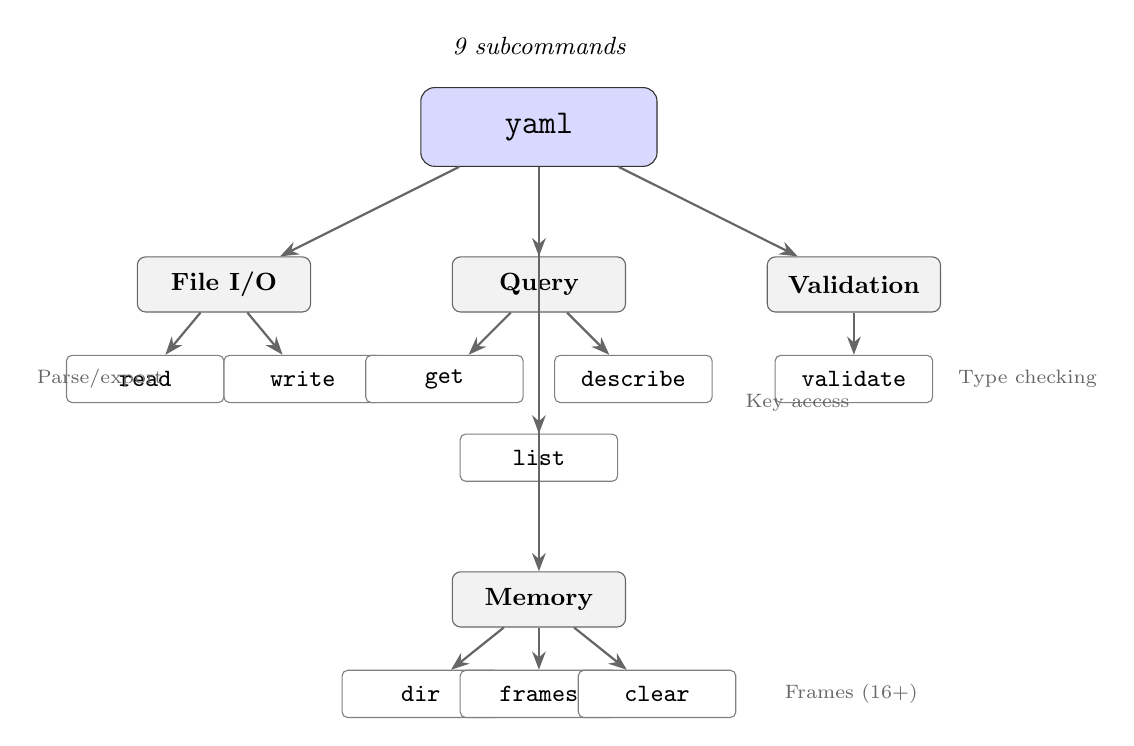
\begin{tikzpicture}[
    % Main command style
    mainbox/.style={
        rectangle, 
        rounded corners=5pt,
        draw=black!80, 
        fill=blue!15,
        minimum width=3cm, 
        minimum height=1cm,
        font=\large\bfseries\ttfamily
    },
    % Subcommand category style
    catbox/.style={
        rectangle, 
        rounded corners=3pt,
        draw=black!60, 
        fill=gray!10,
        minimum width=2.2cm, 
        minimum height=0.7cm,
        font=\small\bfseries
    },
    % Individual subcommand style
    cmdbox/.style={
        rectangle, 
        rounded corners=2pt,
        draw=black!50, 
        fill=white,
        minimum width=2cm, 
        minimum height=0.6cm,
        font=\small\ttfamily
    },
    % Arrow style
    arrow/.style={
        ->,
        >=Stealth,
        thick,
        black!60
    },
    % Brace style
    brace/.style={
        decorate,
        decoration={brace, amplitude=5pt, raise=2pt}
    }
]

% === Main Command ===
\node[mainbox] (yaml) at (0, 0) {yaml};

% === Category: File I/O ===
\node[catbox] (fileio) at (-4, -2) {File I/O};
\node[cmdbox] (read) at (-5, -3.2) {read};
\node[cmdbox] (write) at (-3, -3.2) {write};

% === Category: Query ===
\node[catbox] (query) at (0, -2) {Query};
\node[cmdbox] (get) at (-1.2, -3.2) {get};
\node[cmdbox] (list) at (0, -4.2) {list};
\node[cmdbox] (describe) at (1.2, -3.2) {describe};

% === Category: Validation ===
\node[catbox] (valid) at (4, -2) {Validation};
\node[cmdbox] (validate) at (4, -3.2) {validate};

% === Category: Memory Management ===
\node[catbox] (memory) at (0, -6) {Memory};
\node[cmdbox] (dir) at (-1.5, -7.2) {dir};
\node[cmdbox] (frames) at (0, -7.2) {frames};
\node[cmdbox] (clear) at (1.5, -7.2) {clear};

% === Arrows from main to categories ===
\draw[arrow] (yaml) -- (fileio);
\draw[arrow] (yaml) -- (query);
\draw[arrow] (yaml) -- (valid);
\draw[arrow] (yaml.south) to[out=-90, in=90] (memory.north);

% === Arrows from categories to commands ===
\draw[arrow] (fileio) -- (read);
\draw[arrow] (fileio) -- (write);
\draw[arrow] (query) -- (get);
\draw[arrow] (query) -- (list);
\draw[arrow] (query) -- (describe);
\draw[arrow] (valid) -- (validate);
\draw[arrow] (memory) -- (dir);
\draw[arrow] (memory) -- (frames);
\draw[arrow] (memory) -- (clear);

% === Annotations ===
\node[font=\scriptsize, text=black!60, anchor=west] at (-6.5, -3.2) {Parse/export};
\node[font=\scriptsize, text=black!60, anchor=west] at (2.5, -3.5) {Key access};
\node[font=\scriptsize, text=black!60, anchor=west] at (5.2, -3.2) {Type checking};
\node[font=\scriptsize, text=black!60, anchor=west] at (3, -7.2) {Frames (16+)};

% === Title ===
\node[font=\small\itshape, anchor=south] at (0, 0.8) {9 subcommands};

\end{tikzpicture}

\end{document}
